\documentclass[graphics]{beamer}

\usepackage{graphicx}
\usepackage{verbatim}
\usepackage{wrapfig}
\useoutertheme{shadow}
%\usecolortheme{orchid}
\usecolortheme{seahorse}


% math commands
\newcommand{\be}{\begin{eqnarray}}
\newcommand{\ee}{\end{eqnarray}}
\newcommand{\beq}{\begin{equation}}
\newcommand{\eeq}{\end{equation}}
\def\simless{\mathbin{\lower 3pt\hbox
      {$\rlap{\raise 5pt\hbox{$\char'074$}}\mathchar"7218$}}}
\def\simgreat{\mathbin{\lower 3pt\hbox
      {$\rlap{\raise 5pt\hbox{$\char'076$}}\mathchar"7218$}}} %> or of order

% variables

\def\toonscale{0.45}
\def\mboxy#1{\mbox{\small #1}}


\begin{comment}
\AtBeginSection[]{
  \frame{
    \frametitle{Outline}
    \tableofcontents[currentsection]
  }
}
\end{comment}

\title{Classical Mechanics, Quantum Mechanics, Quantum Cosmology: new view on the universe
}
%\subtitle{interim update}
\author[U. Pen]{Ue-Li Pen (ASIAA and CITA) Dylan Jow (CITA), Job
  Feldbrugge (Edinburgh), TF Jiang (NYCU)
}
\date{January 6, 2023}


\begin{document}

%\section*{Introduction}
\section{Lenses}

\begin{comment}
  \subsection{Outline}

  \frame{
    \frametitle{Outline}
    \tableofcontents
  }
\end{comment}

\frame{\maketitle}



  \frame{
    \frametitle{Waves, Particles, Geodesics}
    \begin{itemize}
        \item Everything is a wave
        \item Short wavelength limit has classical particle
          interpretation: Eikonal
        \item Picard-Lefschetz: no waves, everything is a particle!
        \item New tool for QM Cosmology, FRBs, pulsars
        \item alternative picture for quantization: quantum gravity?
    \end{itemize}
  }

  \frame{
\vspace{-0.25in}
    \frametitle{Fermat's Principle}
    \begin{itemize}
        \item light takes shortest path. Why?
        \item Huygen's principle: light takes all paths
        \item Kirchoff/Feynmann path integral
        \item stationary phase dominates
        \item classical equation of motion: extremal paths, independent of wavelength
\vspace{-0.85in}\hspace{2.5in}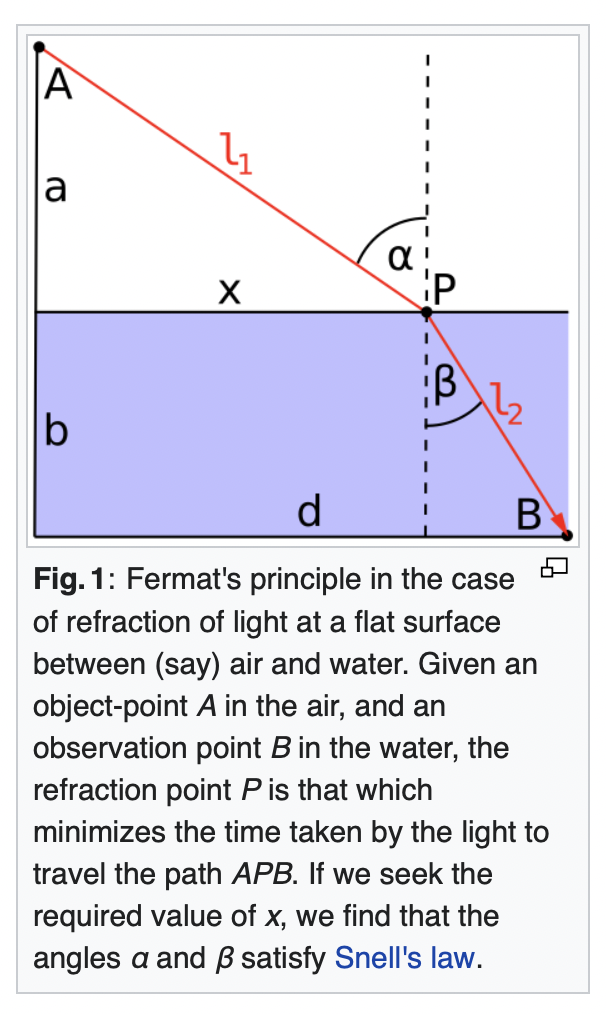
\includegraphics[width=1.3in]{Figures/fermat.png}
    \end{itemize}
  }

  \frame{
\vspace{-0.5in}
    \frametitle{History}
    \begin{itemize}
    \item Huygens, Fermat, Feynmann
    \item Picard-Lefschetz (19th century), Witten (2010)          
    \item concept: Oscillatory (Kirchoff) path integral
    \item sum over all possible paths, weighted by phase
    \item new phenomena: imaginary images, diffraction
    \item Eikonal: Dual description of waves by particles
    \end{itemize}
  }


  \frame{
\vspace{-0.25in}
    \frametitle{Optics: Geometric, Eikonal, Wave, P-L}
    \begin{itemize}
        \item Consider 1-D lens
        \item lensing potential $\Psi(\theta)$
        \item deflection $\Psi'$
        \item simplify for $D_{\rm ds}=\infty$
    \end{itemize}
\vspace{-0.5in}\hspace{2.5in}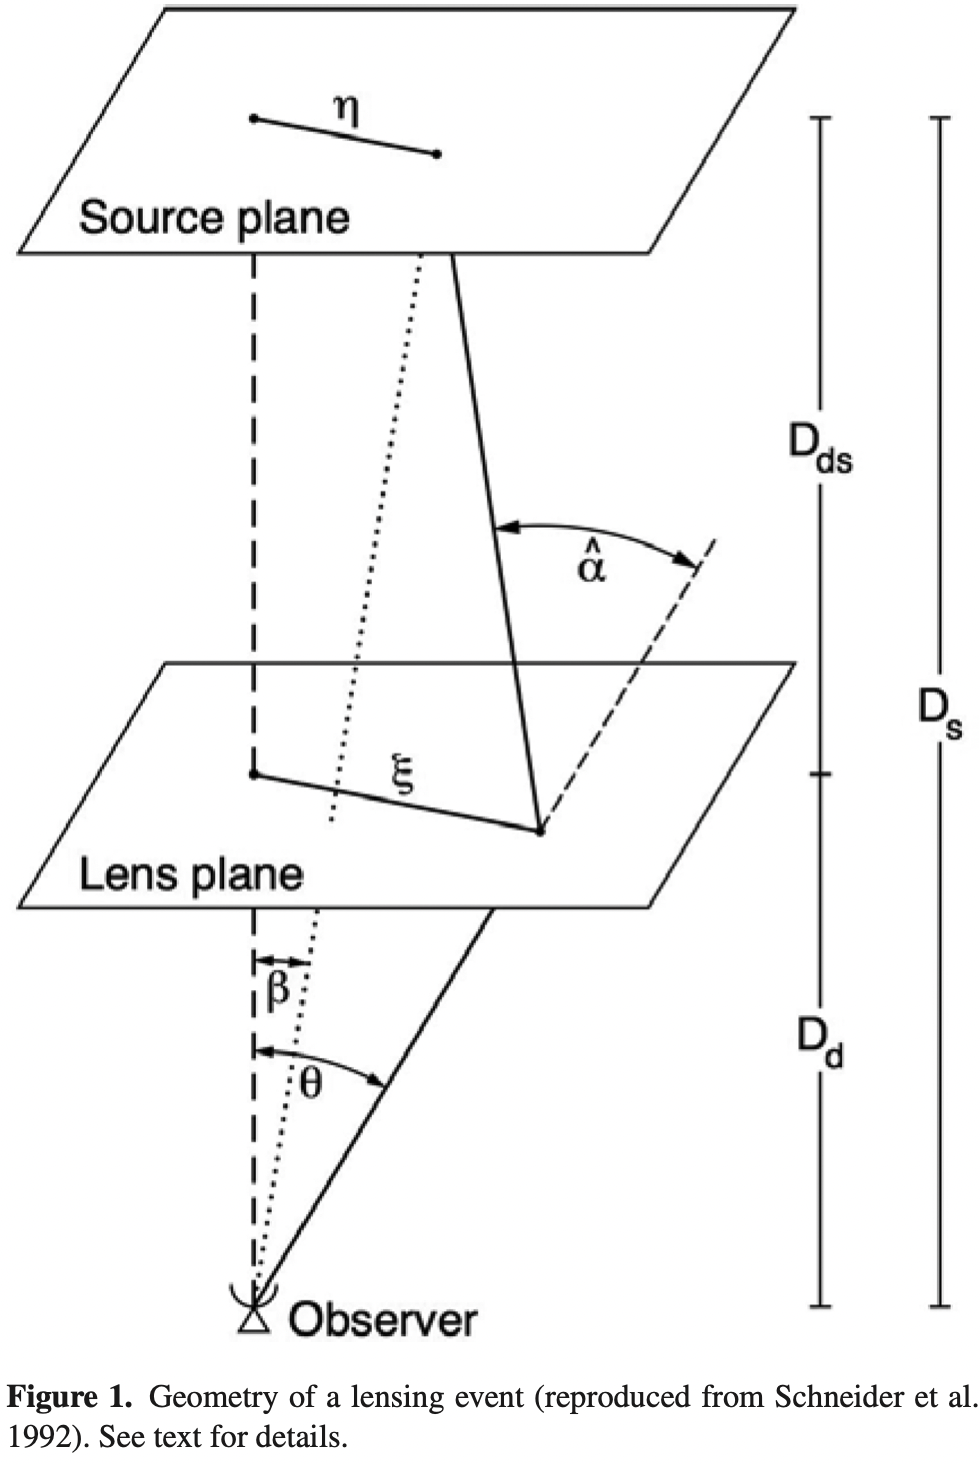
\includegraphics[width=1.5in]{Figures/lens.png}

  }


  \frame{
\vspace{-0.25in}
    \frametitle{Huygen's Principle: Path Integral}
    \begin{itemize}
        \item $A(\mu)=\int e^{i S(\theta,\mu)} d\theta$ 
        \item $S=\nu [(\theta-\mu)^2+\Psi(\theta)]$
        \item Highly oscillatory integral, even for $\Psi=0$
        \item Stationary phase points: $\partial_\theta S=0$ leads to (complex)
          Eikonal images $\theta_i$.
        \item flux/phase through curvature expansion (known as {\it
            steepest descent}): exact as $\nu \rightarrow \infty$
        \item Geometric limit considers only {\it Real} solutions $\theta_i$ and
      gives up phase
          information (length of trajectory)
        \item Geometric optics applicable at short wavelengths for
          extended sources
          (e.g. optical gravitational lensing of finite size sources,
          stars)     
          \item roughly 1/4 of the degrees of freedom of Eikonal 
    \end{itemize}
  }


  \frame{
\vspace{-0.5in}
    \frametitle{Imaginary Images}
    \begin{itemize}
    \item consider ``rational lens'' potential $\psi(\theta)=\alpha/(1+\theta^2)$
    \item Geometric/eikonal images at $\psi'=\theta$
    \item 5 roots.  1 or 3 real roots, rest imaginary
    \item P-L: at most one imaginary image contributes!
    \item imaginary image can be brighter than unlensed real image
    \end{itemize}
  }


  \frame{
%\vspace{-0.5in}
    \frametitle{Rational 1-D lens}
\begin{center}
\includegraphics[width=3.1in]{Figures/theta-beta.eps}
\end{center}
  }

  \frame{
\vspace{-0.5in}
    \frametitle{Picard-Lefschetz Theory}
    \begin{itemize}
    \item descend integral along real line along Morse function Im(S)
    \item contour deforms into finite number of Thimbles of constant
      phase with maximum at saddle point (extrema $dS=0$)
    \item correctly identifies relevant saddle points
    \item resolves numerical challenges of oscillatory integral
    \item complex analysis works in multiple variables
    \item elevates concept of ``image'' deep into wave optics
    \item multiple public implementations (Feldbrugge+, Jow+)
    \end{itemize}
  }



  \frame{
\vspace{-0.5in}
    \frametitle{Picard-Lefschetz Theory}

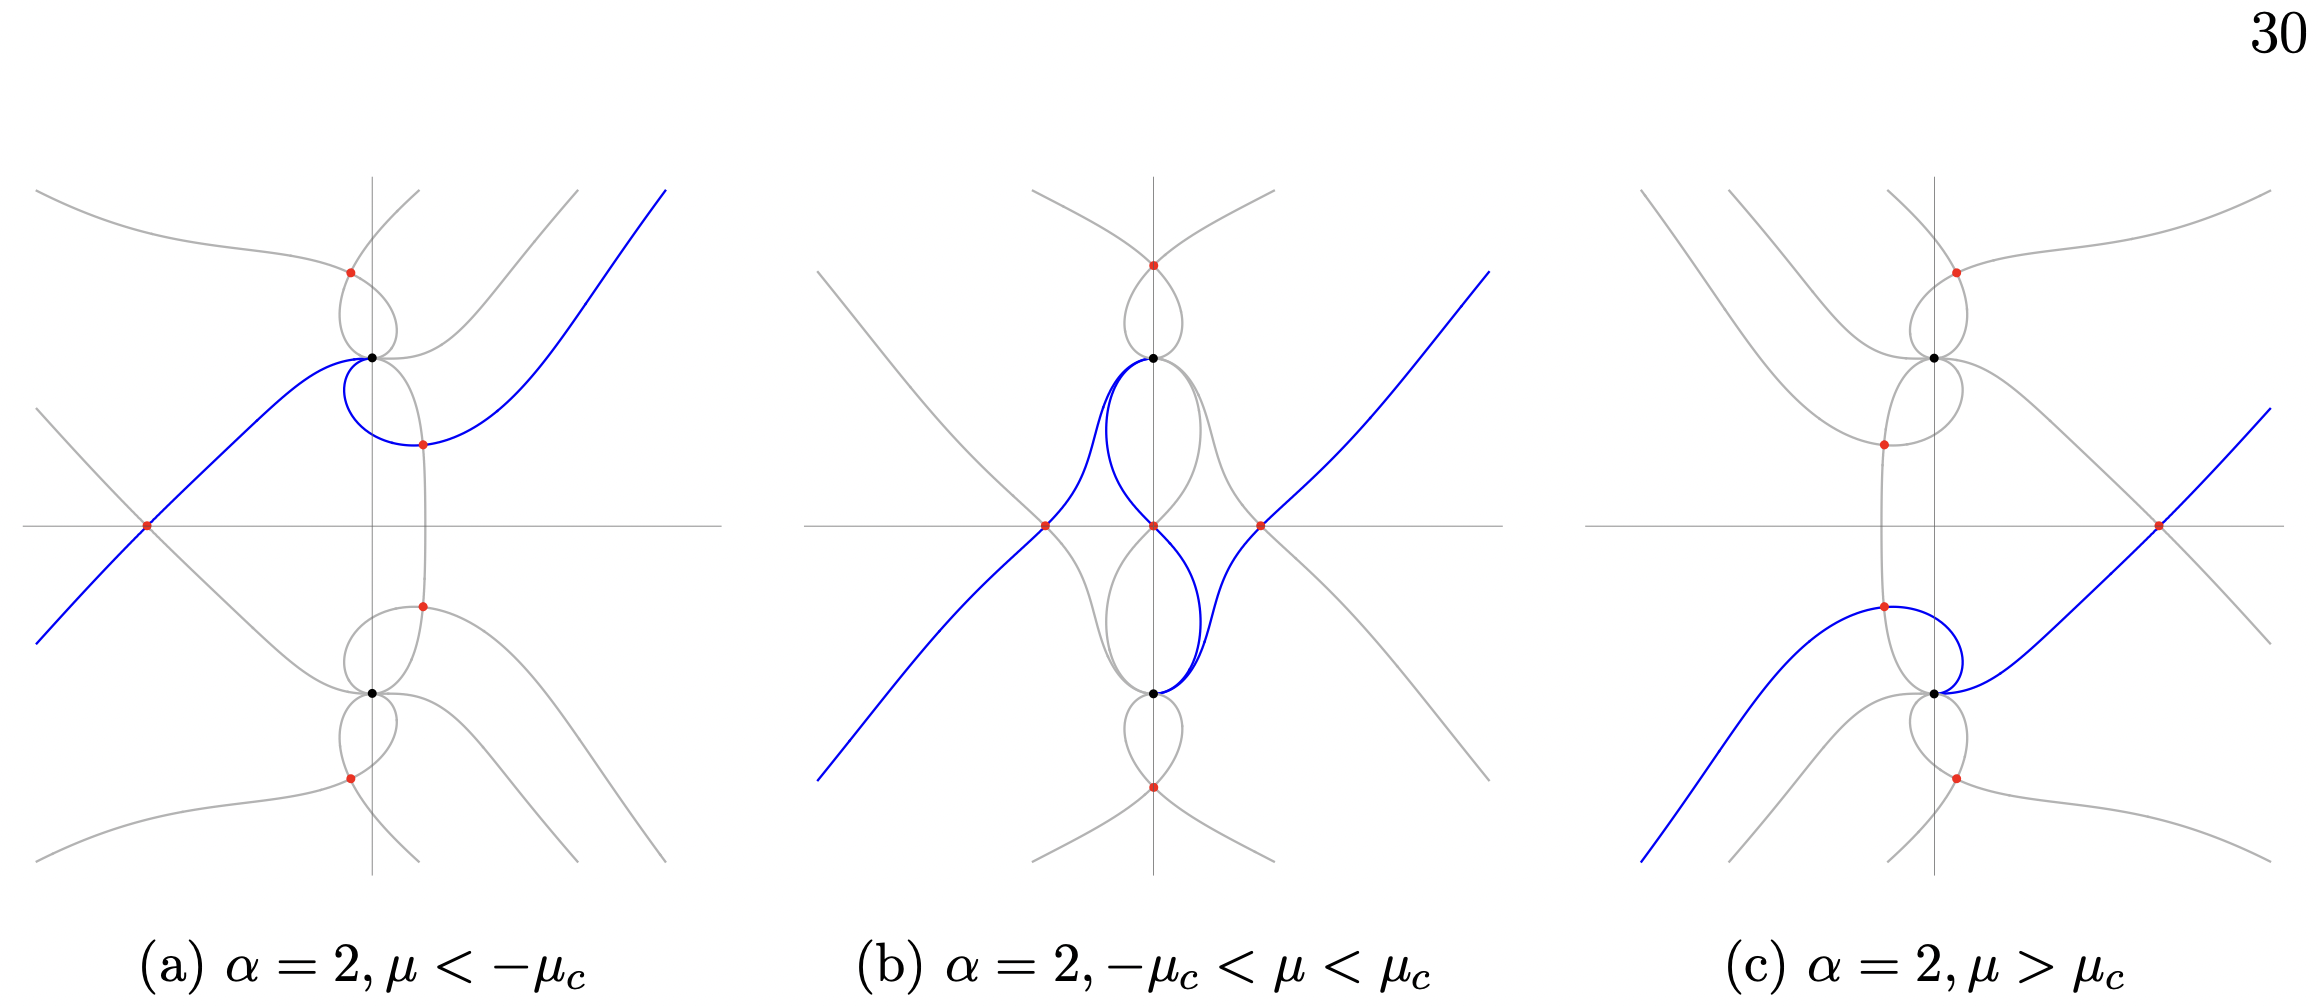
\includegraphics[width=4.5in]{Figures/thimbles.png}

Feldbrugge+2019
  }


  \frame{
\vspace{-0.5in}
    \frametitle{Imaginary classical paths}
    \begin{itemize}
    \item PL interpretation: oscillatory integral is sum over thimbles
    \item each thimble has exactly one stationary point (maxima, classical path)
    \item path integral is sum over thimbles
    \item eikonal limit is quadratic expansion at maxima (WKB for
      imaginary images)
    \item alternative interpretation of quantum mechanics from
      classical mechanics:
    \item sum over real and imaginary classical paths
    \item Turok 2014, Cherman+ 2014, Mou+ 2019
    \end{itemize}
  }

  \frame{
\vspace{-0.5in}
    \frametitle{New Observables}
    \begin{itemize}
    \item for coherent sources: FRBs, pulsars
    \item weak lensing: imaginary image allows time delay measurement (Jow+21)
    \item strong lensing: delay measurements enable measurement of
      co-linearity (Jow++21)
    \item microlensing: instant time delay, planets (Jow+20)
    \item macrolensing: potentially nano-second delay -- universe
      expands!  Dark energy, etc (Wucknitz+21)
    \item dimensionless strain cm/Gigalightyears $h\sim \Delta t/t \sim 10^{-26}$:
      competitive with LIGO, etc
    \end{itemize}
  }


  \frame{
%\vspace{-0.5in}
    \frametitle{A2 fold}
\begin{center}
%\vspace{-0.3in}
%\hspace{-1.2in}
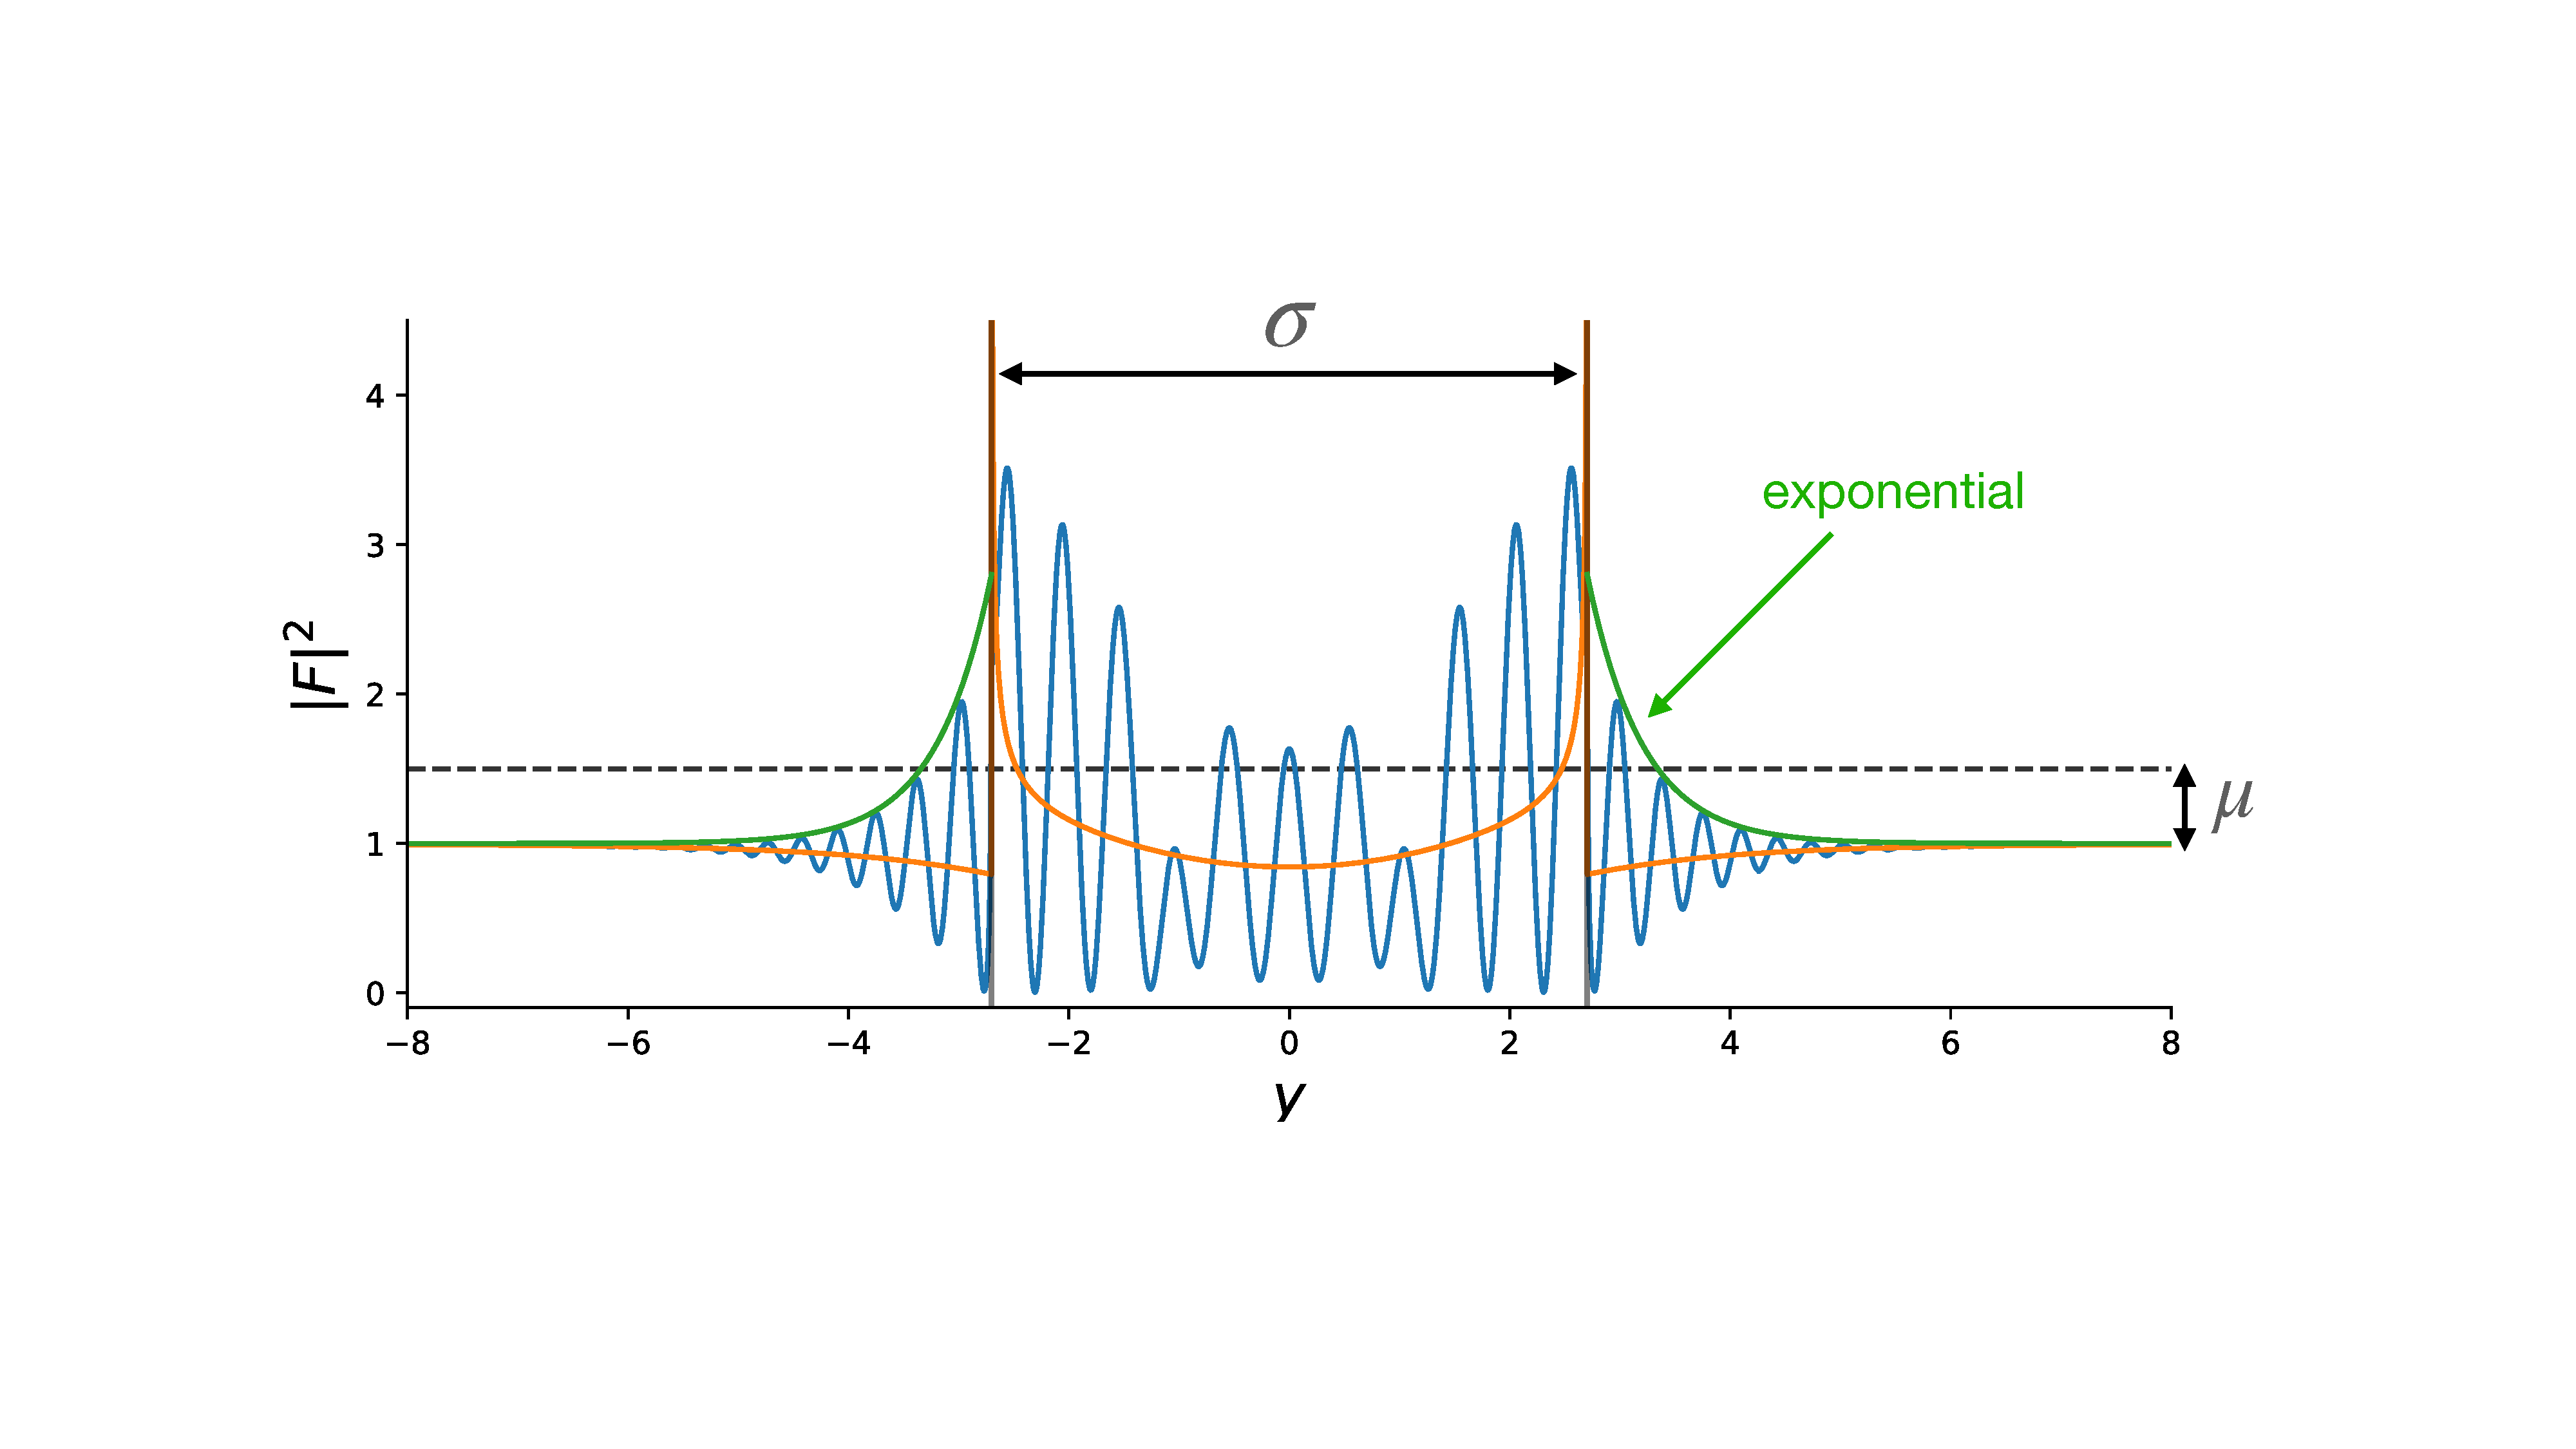
\includegraphics[width=4.5in]{Figures/flux_diagram.pdf}
\end{center}
  }


  \frame{
\vspace{-0.5in}
    \frametitle{Feynman Path Integrals}
    \begin{itemize}
    \item local description of wave function, equivalent to solving
      Schroedinger equation
    \item $\Psi(x_f,t_f)={\cal N} \int Dx \int dx_i e^{{i\over \hbar}S
        (x_f,t_f,x_i,t_i) }\Psi(x_i,t_i)$
    \item full solution, not perturbative
    \item more general for unbounded Hamiltonians
    \item PL: maps to discrete set of complex paths
    \end{itemize}
  }

  \frame{
%\vspace{-0.5in}
    \frametitle{P\"oschl-Teller Potential}
\begin{itemize}
\item $V(x)={\rm sech}^2(x)$
  \item  exactly solvable: 
$\sinh[x(t)]=\sqrt{\frac{1-E}{E}} \cosh[\sqrt{E}(t+t_0)]$
    \item for $\lim_{E\rightarrow 1+\epsilon^2} = \sinh^{-1} [\epsilon \sinh(t)]$
    \end{itemize}
 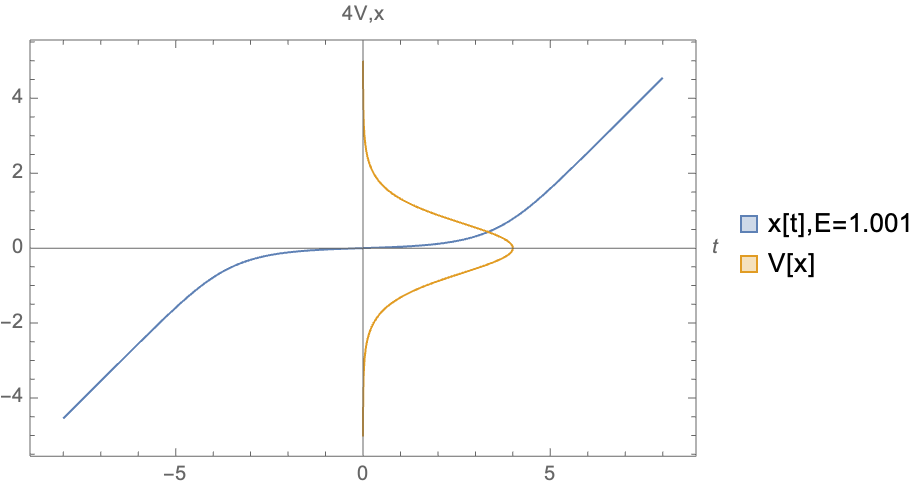
\includegraphics[width=3.5in]{Figures/sechreal.png}
  }


  \frame{
\vspace{-0.5in}
    \frametitle{P\"oschl-Teller Potential}
\begin{itemize}
\item $V(x)={\rm sech}^2(x)$
  \item  exactly solvable: 
$x(t)=-i \sin^{-1}\left[\sqrt{\frac{1-E}{E}}\sinh(\sqrt{E}t)\right]$
    \item for $\lim_{E\rightarrow 0} = -i\sin^{-1}(t)$
    \end{itemize}
 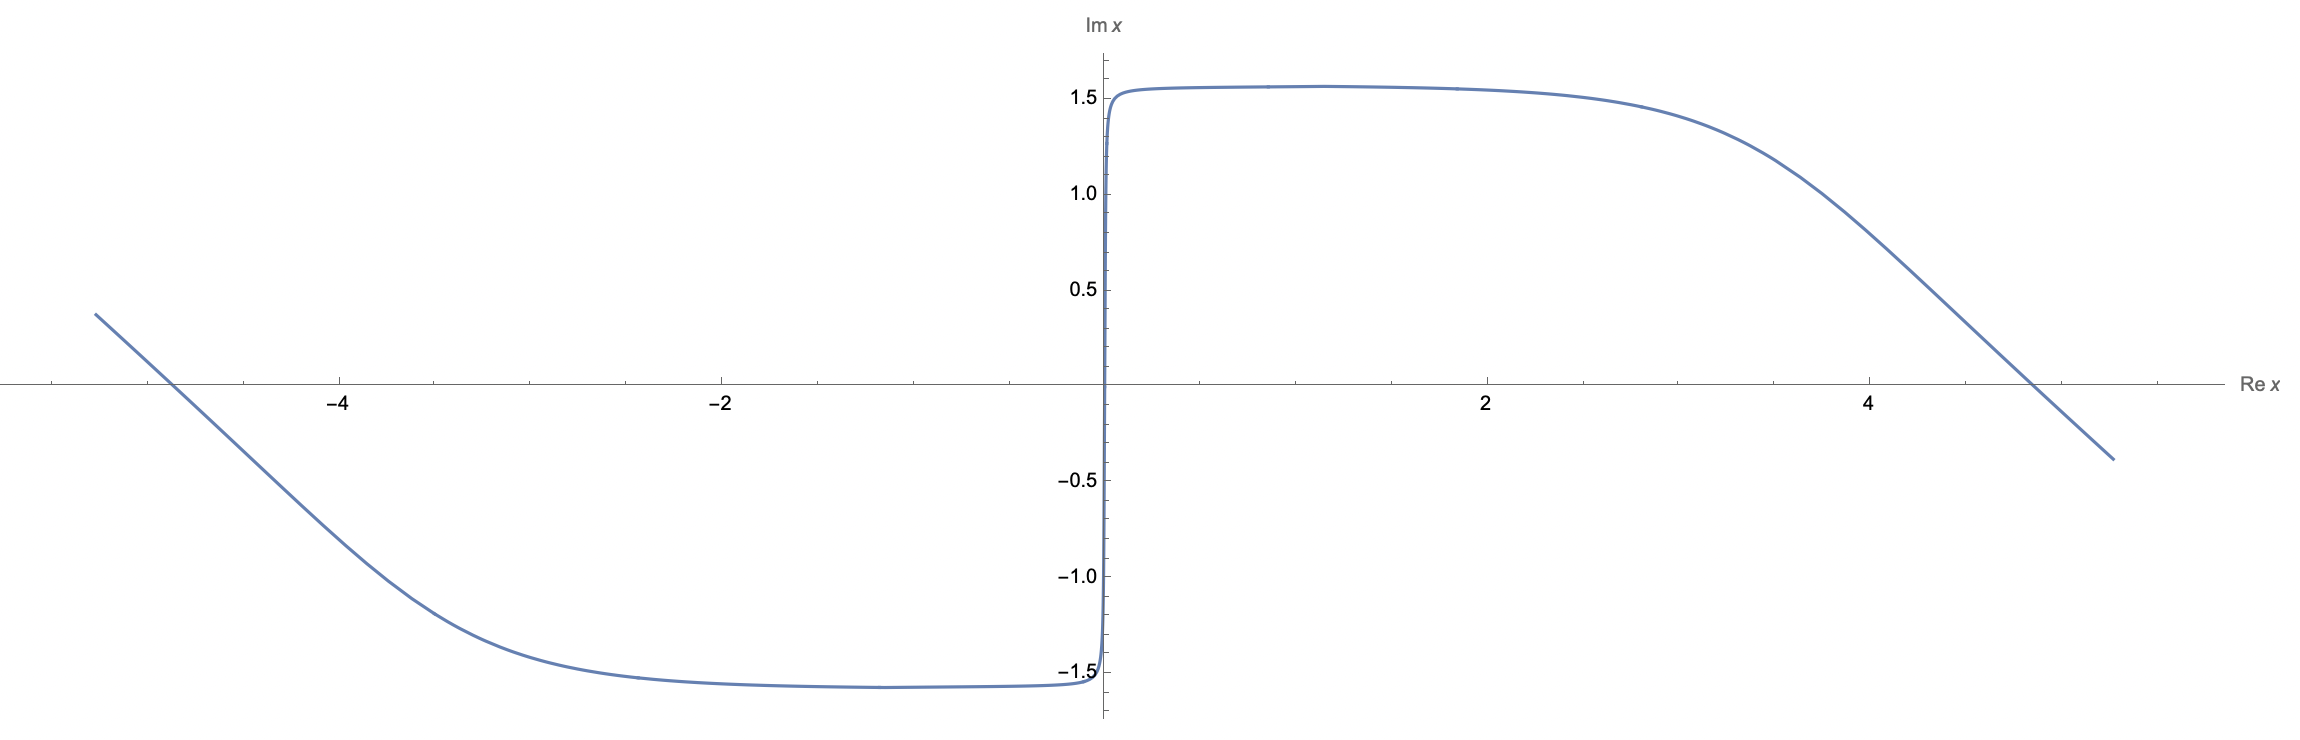
\includegraphics[width=4.5in]{Figures/sechtunnel.png}
  }


  \frame{
\vspace{-0.5in}
    \frametitle{Lorenzian Quantum Cosmology}
    \begin{itemize}
    \item Feldbrugge, Lehners \& Turok 2017
    \item Quantize Feynmann path integral instead of wave equation
    \item PL, Cauchy's theorem allow deformation of paths into complex plane
    \item minisuperspace: allow imaginary paths (scale factor)
    \item PL Semi-classical limit: dominant paths
    \item CPT universe, bounce, etc (Boyle, Finn, Turok 2018)
    \end{itemize}
  }



  \frame{
\vspace{-0.5in}
    \frametitle{Discussion}
    \begin{itemize}
    \item Eikonal effects applicable to compact radio sources,
      e.g. FRBs, pulsars
    \item full wave
effect dominates for long wavelengths as Fresnel scale is bigger then Einstein radius
    \item down to planet size
    \item gravitational waves:  LIGO, LISA, PTA
    \end{itemize}
  }





\frame{
    \frametitle{BURSTT}
Bustling Universe Radio Telescope Taiwan: collaboration of ASIAA, NTU,
NTHU, NCHU for all sky FRB radio array
     \hspace{-0.5in}
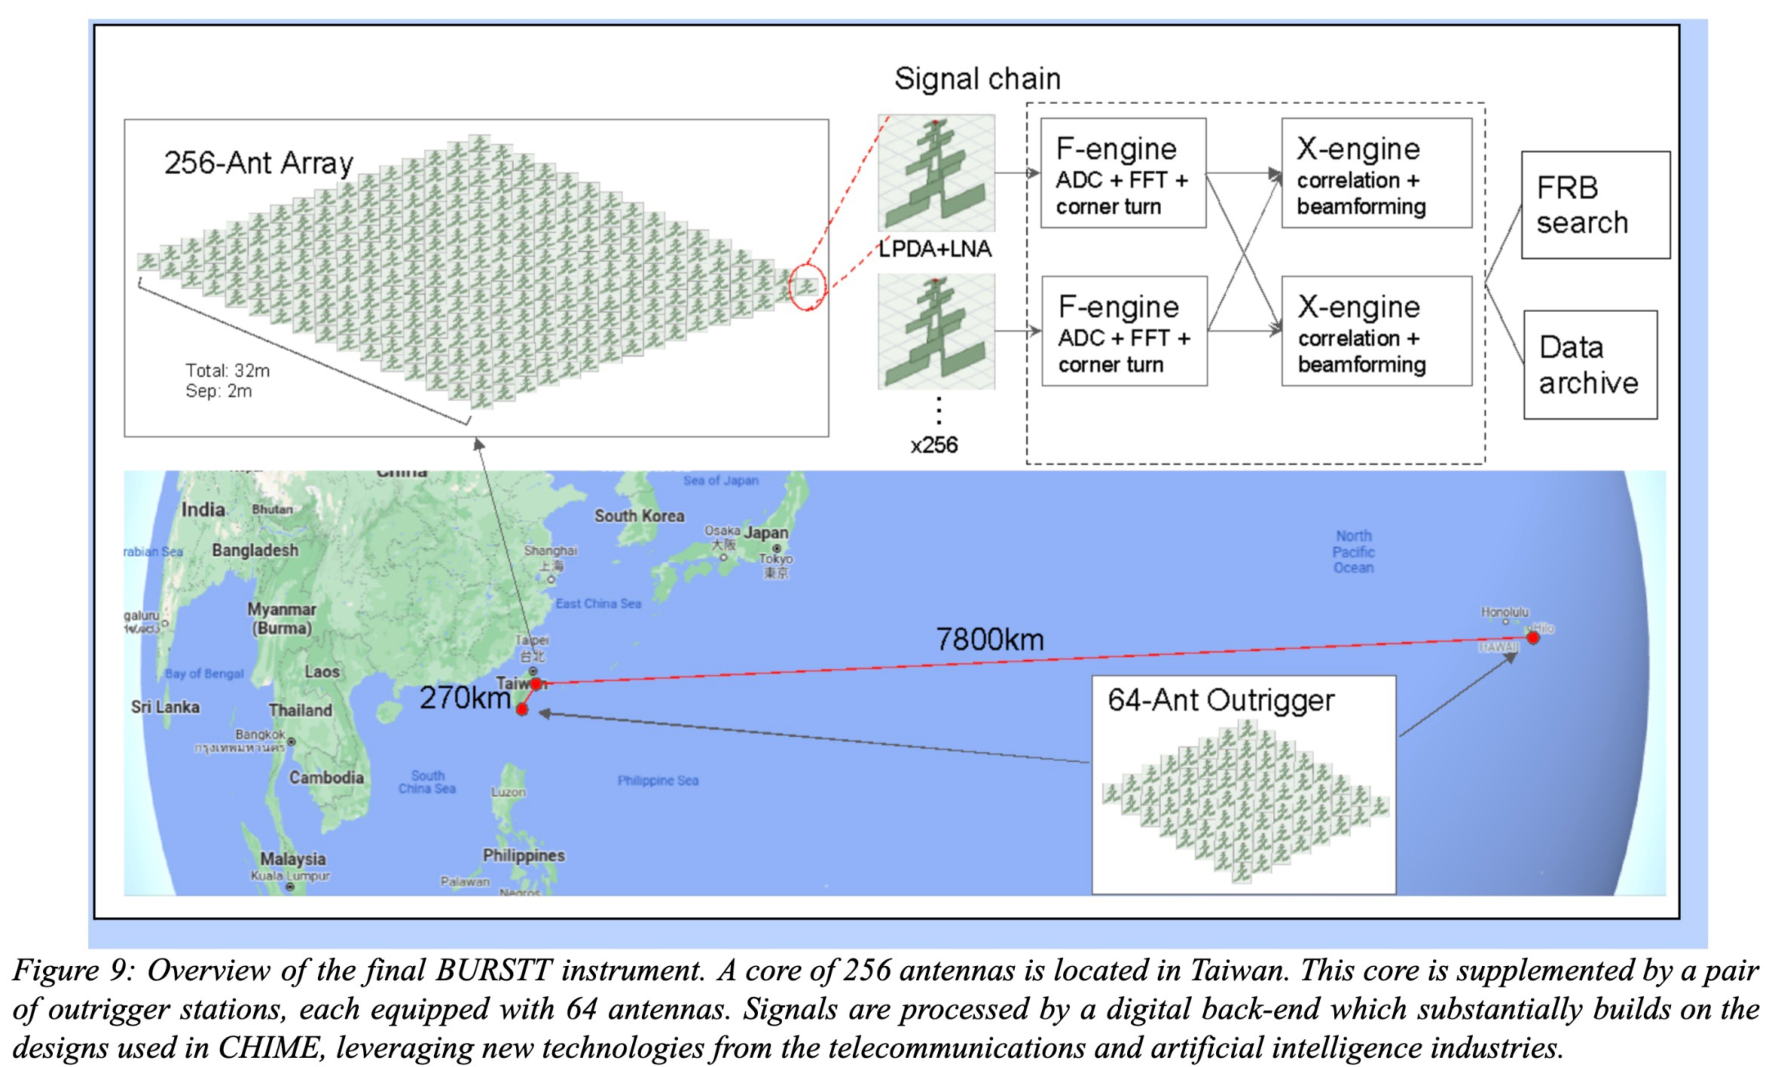
\includegraphics[width=0.55\textwidth]{Figures/BURSTT.pdf}
\includegraphics[width=0.45\textwidth]{Figures/fushanplatform.jpeg}


}


  \frame{
\vspace{-0.5in}
    \frametitle{Conclusions}
    \begin{itemize}
    \item Picard-Lefschetz theory provides alternative interpretation
      of optics, quantum mechanics: imaginary positions and trajectories
    \item wave optics changes nature of astrophysical observables: Coherent FRB
      radiation one of the potentially most
      precise measurements in physics.  Imaginary images extends
      classical tools to include full wave optics: time delay
      measurements in weak lensing
    \item new tool to compute quantum gravity, bypassing historical conceptual barriers.
    \end{itemize}
  }

\end{document}
